\chapter{Design and Implementation}
\label{chap_impl}

This Chapter deals with the implementation of \textit{This is How} including Technology and User experience. It also includes a section dedicated to SuperGlue, the automatic metadata extraction system, including description and implementation, 

\section{Technology Considerations}

Given that \textit{This is How} caters to makers and hackers, the technology stack it employs should respect their values of openness and transparency. As such, it must be coherent, extensible and modifiable.
 
\textit{This is How} is developed as an open source project. The source code has been and will continue to be available throughout all stages of development, not just on release, and allow for community contributions. It utilizes open standards, these are governed by transparent standard committees and are royalty free. 

\textit{This is How} allows for rapid iterative development. This means it uses programming languages, libraries and frameworks that value productivity over other considerations such as performance. This also derives extensibility, it allows for simple integration and composition of third-party open source packages. 

\textit{This is How} is built with familiar tools. While it is sometimes tempting to use niche programming languages and technologies, these interfere with the ease of community contribution. I prefer technologies with a proven track record and wide adoption rates.

\section{Technology Details}

\textit{This is How} is developed under the MIT open source license. It is version controlled with the open source GIT\cite{git} version control system and hosted on Github\cite{github} which also tracks bug reports. 

\textit{This is How} is developed as a web application with three major components: server, client and storage. Both the client and server utilize Javascript as their main programming language. The server side uses Node.js, a widely adopted Javascript runtime engine. npm\cite{npm}, the most popular Javascript package manager, is used both as a dependency manager and a build system. The server also uses SuperGlue, described later in this chapter, for video metadata extraction.

ReactJS is The main framework used on the Client side. React provides a component based, efficient rendering engine and as of writing, is the fastest growing web framework \cite{reactjs}. As with the server, NPM manages dependencies although the build process is managed by Webpack \cite{webpack}. For video playback we use the HTML5 <video> tag and for video encoding, the open VP8\cite{vp8} codec. 

Collaborative document editing is done with Etherpad\cite{etherpad}. Etherpad is a collaborative document editor that was launched in 2008 and released as opensource after being acquired by Google in 2009. It has been in development ever since and is extremely flexible. It can work with a variety of datastores, has built in chat and can be easily embedded into other websites.

Storage is divided into structured and unstructured data. The Structured data includes all conversation and metadata while unstructured data refers to the video files. For structured data we use CouchDB\cite{couchdb}, a simple document driven database which allows for real time synchronization between the different clients and the server.  Video files are stored in a simple local file server but can easily plug into 3rd party services such as AWS S3 or Google Cloud Storage.

The Webapp is currently stored on Heroku\cite{heroku}, a popular platform service that makes it simple to deploy new versions and scale up and down. However, the usage of open standards and technologies make it possible to migrate to other services or dedicated hardware as needed. 

\section{SuperGlue - Automatic MetaData extraction}
SuperGlue\cite{superglue} is an automatic metadata extractor that works with all forms of media: video, text and sound. It is a core project and an ongoing research effort at the Viral Communications group. The current iteration was developed by a team lead by myself and it serves as basis for exploration of media, mostly news, and enables a next generation of media-centered application. (see \autoref{fig_wallofnow})

   \begin{figure}[thpb]
      \centering
      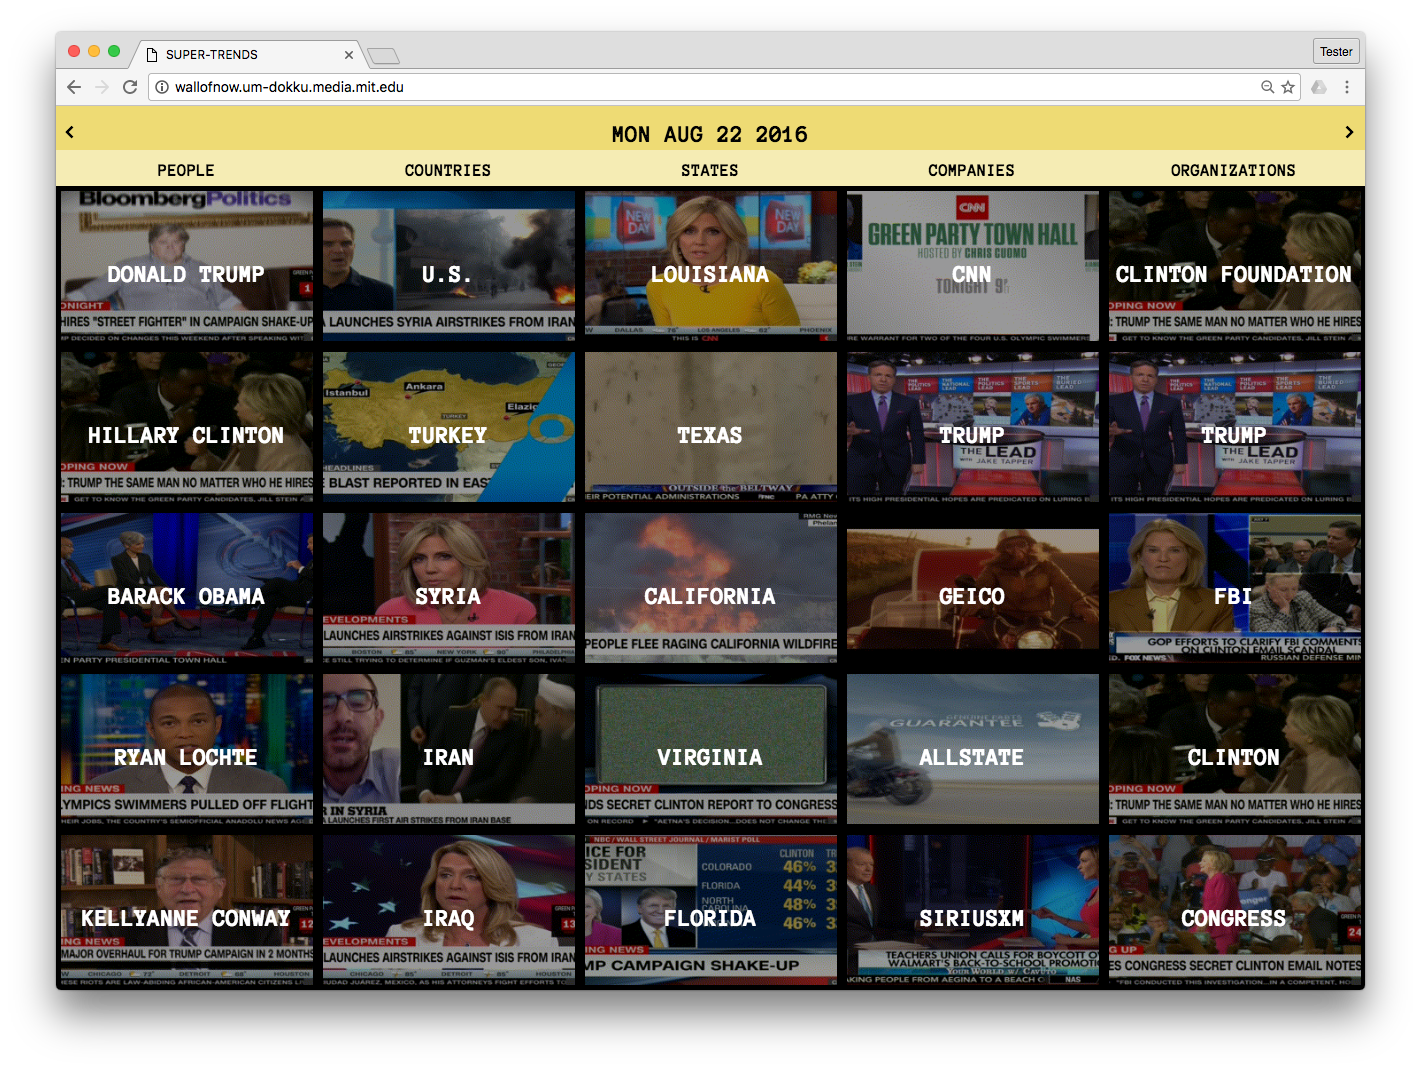
\includegraphics[width=\textwidth]{figures/wallofnow.png}
      \caption{Wall of Now\cite{wallofnow2016} is a project thats displays a digest of the last 24 hours of media from 20 different news channels, using metadata collected by SuperGlue.}
      \label{fig_wallofnow}
   \end{figure}


SuperGlue is built as a modular, expandable system that forms an analysis pipeline. Media is submitted on one side of the pipe and at its end, a rich metadata document is generated and stored on a shared databases. The modules themselves range from face detection to transcription and natural language processing. Modules can declare dependencies on other modules. For example, the natural language keyword extraction module depends on the output of transcription module.

While originally being designed for processing of news, as demonstrated in \textit{This is How}, SuperGlue can handle various types of Media. For This is How, we utilize the keywords extracted from from transcript. From empirical testing, we've concluded these tend to have a high relevance score.    

\subsection{SuperGlue Implementation}

Superglue has four main components: an API server, a task queue, workers, and a datastore. 

The API server is a simple web application written in Python. It's job is to mediate between the application that use SuperGlue as well as receive submissions of new media items and placing them in the task queue. 

The task queue is implemented as a Redis database with one value: a simple ordered list of tasks. Each task represents one module that needs to run on one media item. These tasks are inserted either by the API server or the workers. 

The Workers are the main work horse behind the system and are also implemented in Python. Modules are defined with python classes that adhere to a simple module api. As part of the definition, they can also declare dependencies on other modules. Whenever a worker is free, it polls the task queue for the next task. It then executes the relevant module on the relevant media item and stores the result in the database. Upon completion, it will detect which modules depend on the one that just completed, and will insert new tasks for all of them in the task queue. 

% <TODO: add an illustration of SuperGlue>

All the data is stored in a single collection in a MongoDB database. Each record in this collection represents a single media item and all the output that's been gathered from the various modules is stored in it. 

This architecture results in an ability to successfully scale horizontally. Workers, which are the main units of computation, are stateless and as such can be added and removed without affecting the system. SuperGlue is currently processing 500 hours worth of video in a day using 20 workers running on virtual machines.

\section{User Experience Considerations} 


%    \begin{quotation}
%    ``A user interface is like a joke, If you have to explain it, it's not that good.''
%    \end{quotation} 

% \begin{right}
%     --- Jess Hamilton, Sr. UX/UI Designer at GoPro \\ \medskip
% \end{right}


\begin{flushright}{ \slshape    
    A user interface is like a joke, If you have to explain it, it's not that good.
    } \\ \medskip
    --- Jess Hamilton, Sr. UX/UI Designer at GoPro
\end{flushright}


The user experience of \textit{This is How} is based on the three-step process outlined in the previous chapter: discovery, interactive exposition and collaborative Brainstorming. It must be intuitive and rely mostly on common interaction patterns that users are already accustomed to. When introducing novel ideas they must be as self explanatory as possible. 

\section{User Experience Overview}

In this section I present the major concepts of the user experience. For each page of the interface I present the purpose and an overview of the different components. 

\subsection{Main Concepts}

These concepts are used throughout the user experience. Concepts that are local to a specific portion of the experience will be covered in the relevant section.

\begin{itemize}
\item \textit{Users} are either makers or nonprofits seeking help.

\item \textit{Stories} are the main entity of the system. Each Story has a main video that describes a process and challenges. Stories also encompass the different collaboration concepts that will be described later.

\item \textit{Tags} are terms that represent metadata stories. Each story contains one or more tags. Tags can be manually entered or auto extracted. 
\end{itemize}


\subsection{Main Page}

   \begin{figure}[thpb]
      \centering
      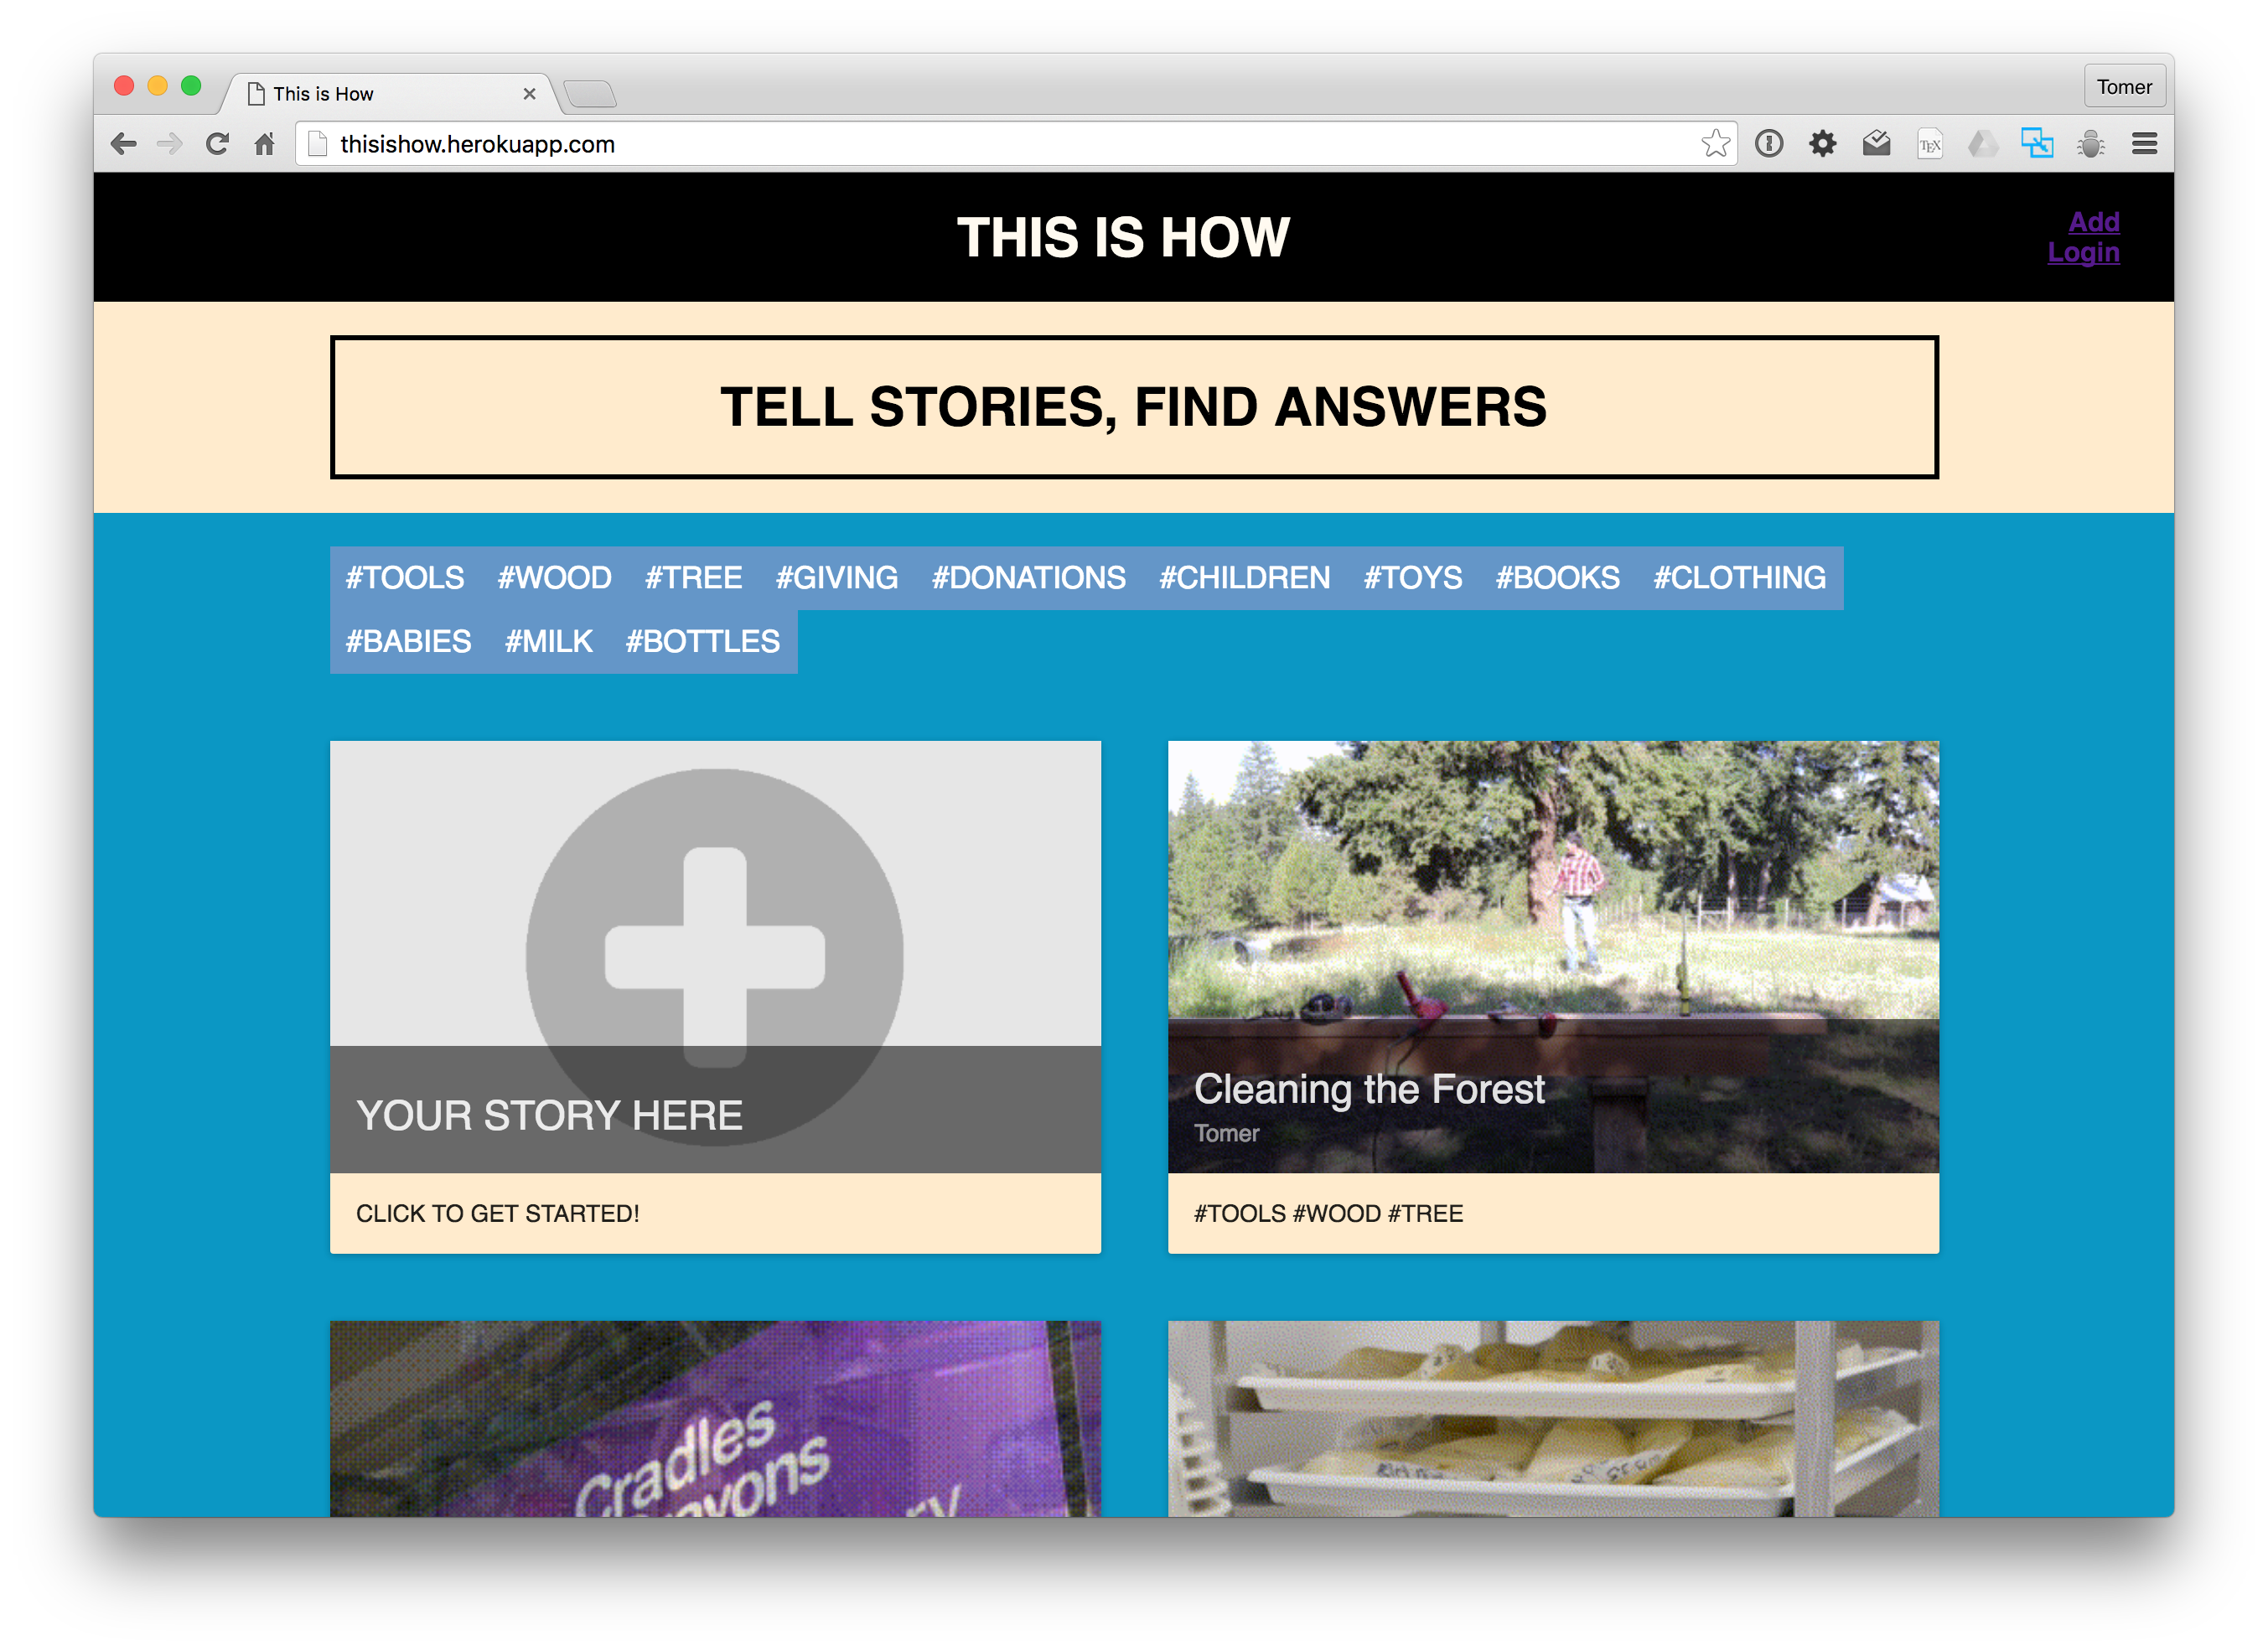
\includegraphics[width=\textwidth]{figures/mainpage.png}
      \caption{This is How - Browsing/Filtering}
      \label{fig_main_page}
   \end{figure}

The main page serves as an entry page for the system. It allows for browsing stories and filtering by tags. All stories are presented, sorted by the time of their addition on a descending order. These stories are represented as thumbnails with some basic data about the story - title and tags. Clicking on the thumbnail will lead to the story page. In later versions, these stories will be sorted by their level of activity, indicated by volume of recent activity and publication date. 

The main page also allows for filtering. A set of common tags is provided, by clicking on a tag, only the stories with a matching tag will be shown. The first story thumbnail is the add button - Hinting that the user can have their story on this page. Clicking it leads to the Add Story Page

\subsection{Add Story Page}

   \begin{figure}[thpb]
      \centering
      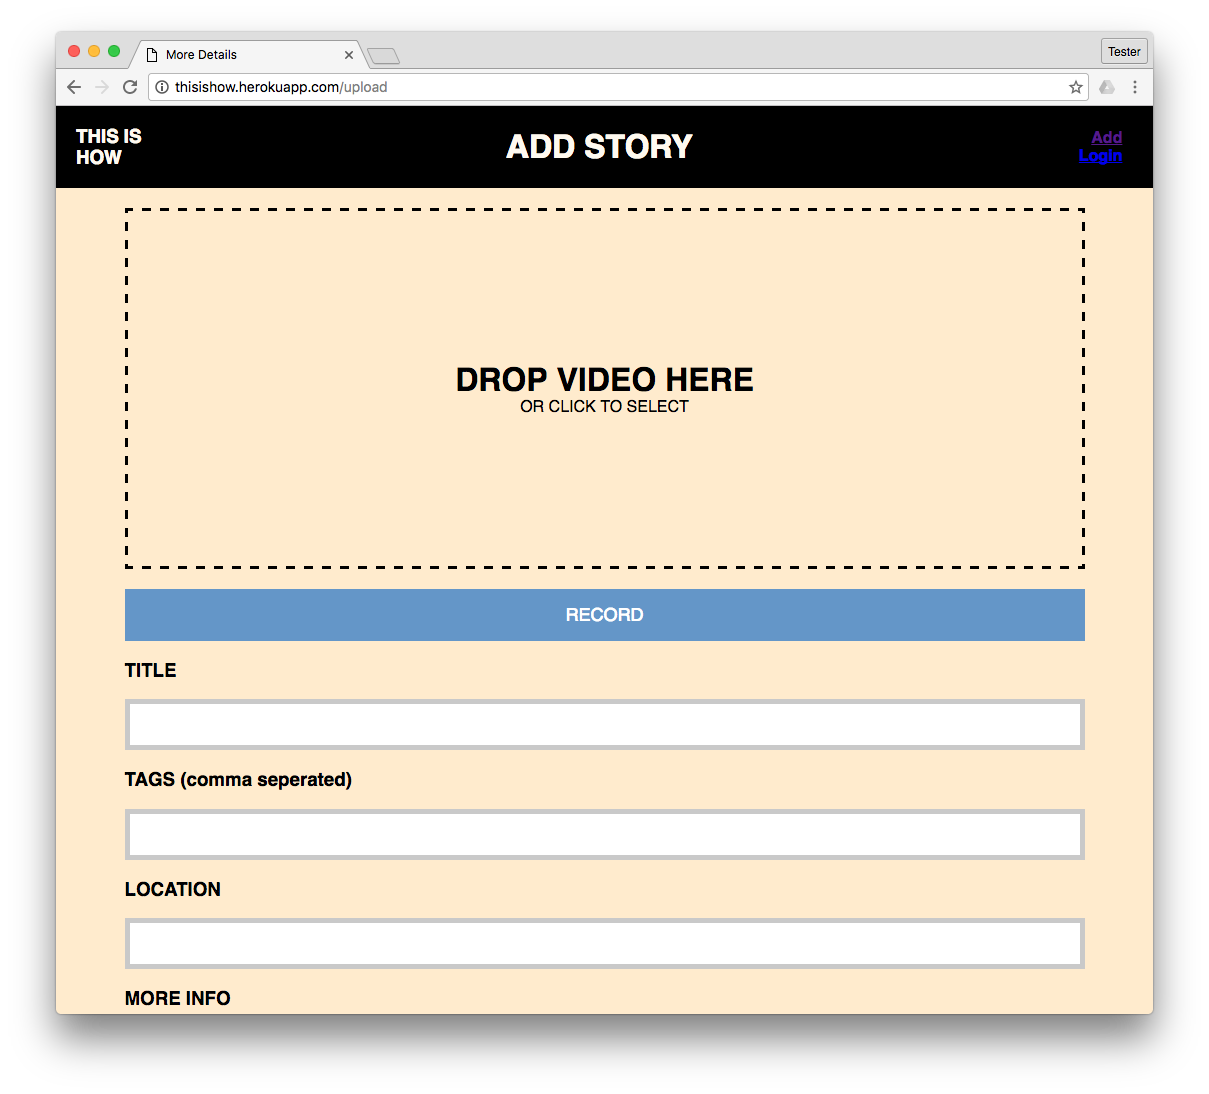
\includegraphics[width=\textwidth]{figures/addstory.png}
      \caption{This is How - Add Story}
      \label{fig_add_story}
   \end{figure}

The Add Story page provides the necessary mechanism for adding a story: uploading a video and providing the necessary details.Video can be uploaded either by clicking on the video area and selecting a file, dropping a video file in it or recording an on-the-fly video, using an attached webcam, by clicking on the \textit{Record} button. Additional data: title, location, description and an initial set of tags, are also required. Clicking the \textit{Publish Now} Button will finalize the process and take the user to their dashboard page. 

\subsection{Dashboard Page}

   \begin{figure}[thpb]
      \centering
      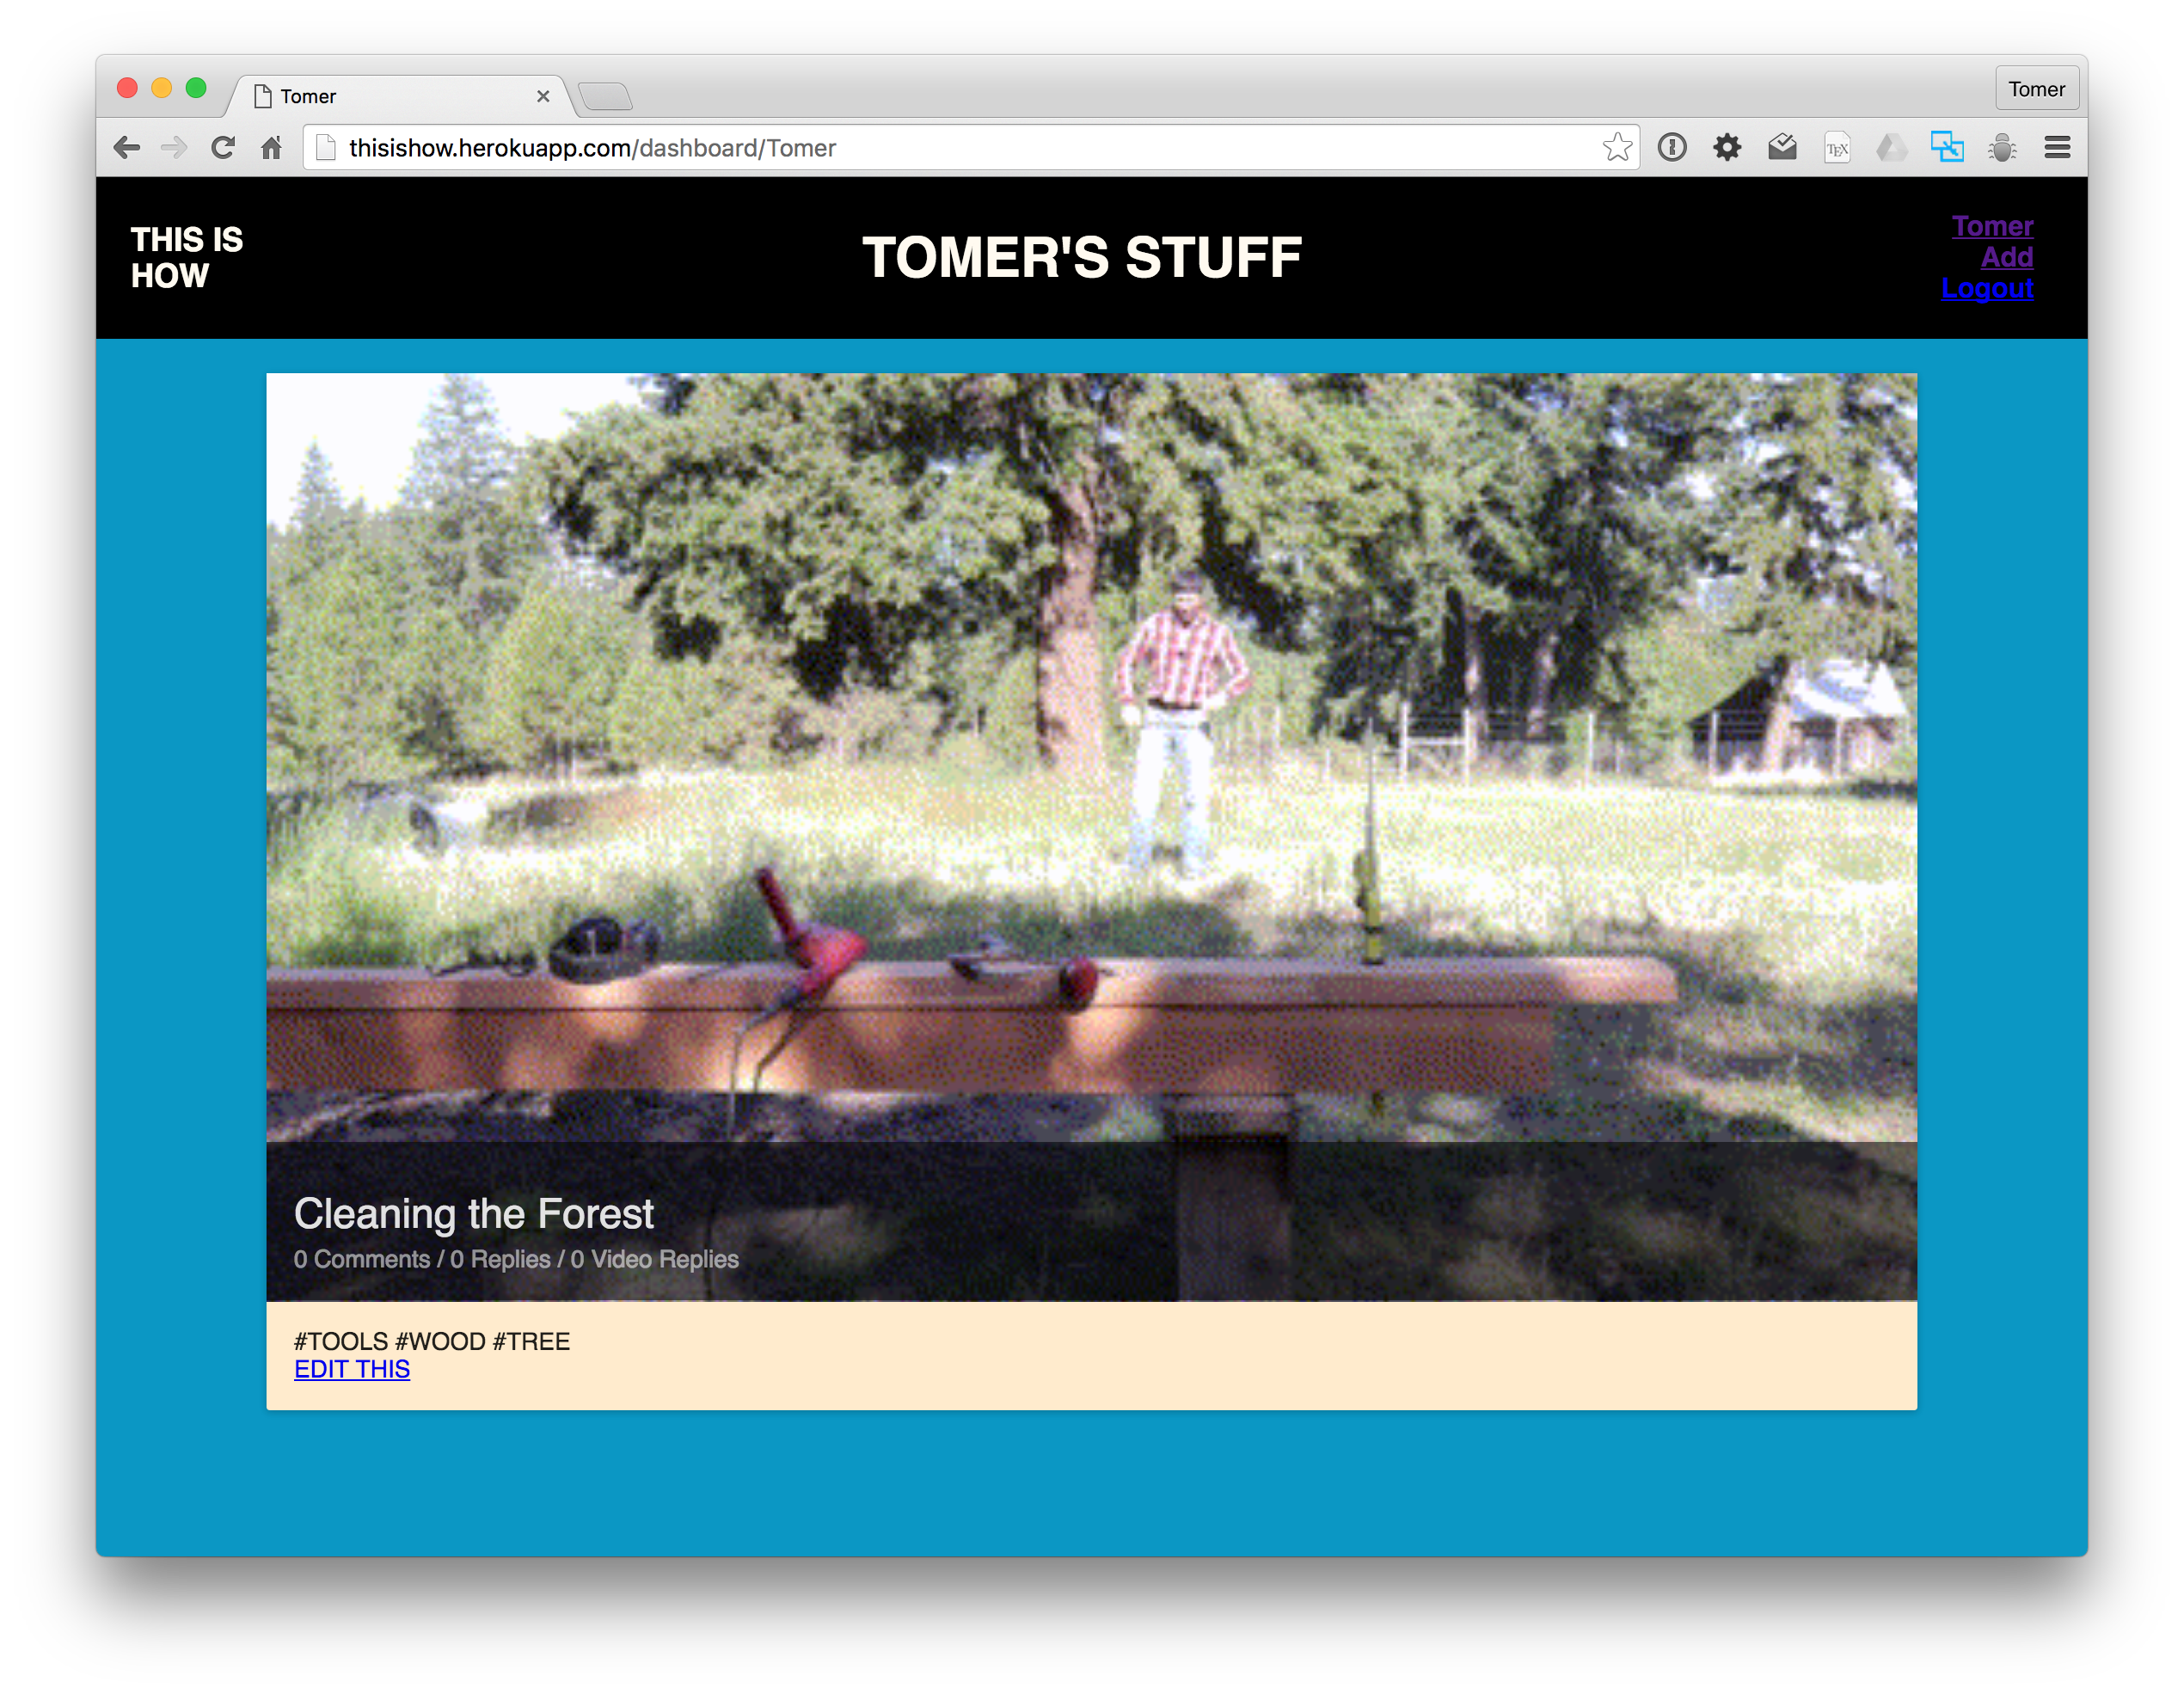
\includegraphics[width=\textwidth]{figures/dashboard.png}
      \caption{This is How - Dashboard}
      \label{fig_dashboard_page}
   \end{figure}

The Dashboard Page is unique per user and presents a collection of all of their published stories. These are shown as story thumbnails, similar to the ones in the main page. Clicking on any story leads to it's story page. 

\subsection{Story Page}

   \begin{figure}[thpb]
      \centering
      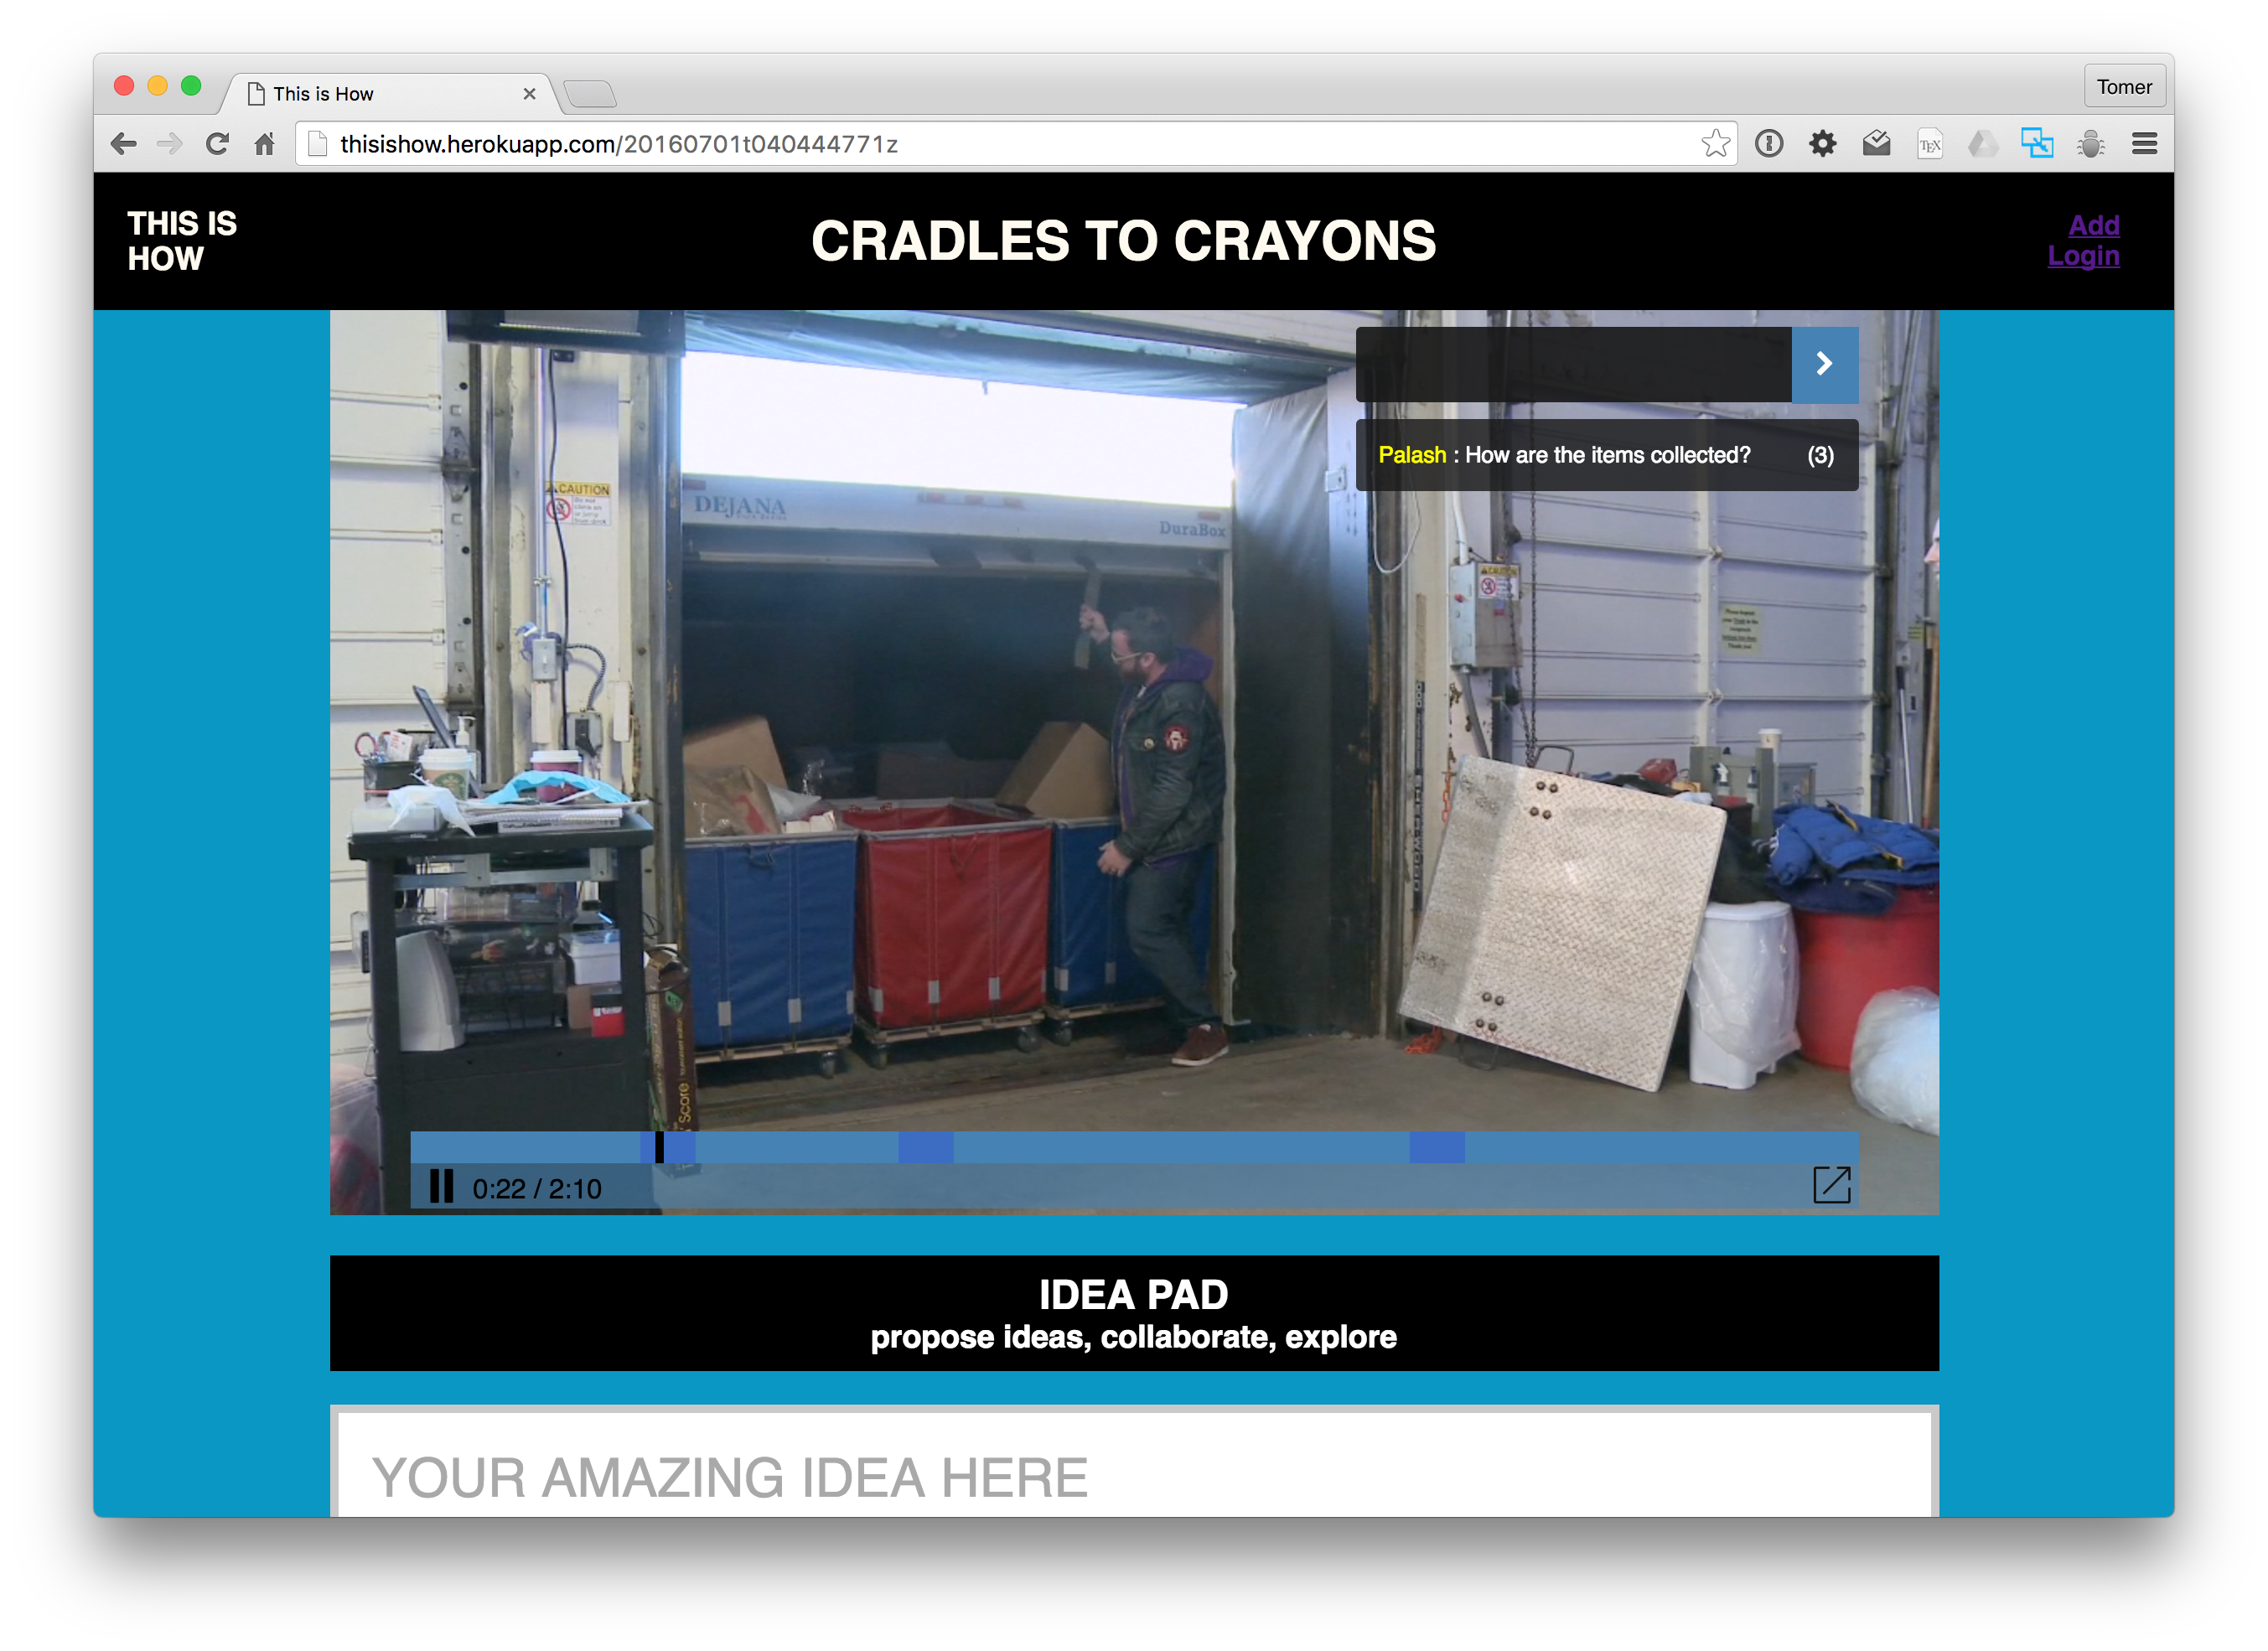
\includegraphics[width=\textwidth]{figures/storypage.png}
      \caption{This is How - Story Page}
      \label{fig_dashboard_page}
   \end{figure}

The Story page is the main tool for facilitating interactive exploration and brainstorming. It consists of two main components: the video component and the idea pad.

\subsection{Video Player}

The video player implements the hyper discussion layer I proposed in the previous chapter. Its basic playback functionality is similar to that of a traditional video player. A seek bar allows for seeking to specific parts in the video and includes a play/pause button and playback time indication.

The video player also includes an always-visible comment input box. When typing a comment, the playback automatically pauses and resumes when the comment is submitted. The submitted comment will be timestamped with the current playback time. Comments appear during playback at their respective timestamp and disappear after a predecided number of seconds. These comments allow participants to contextually ask questions and drill down into the specifics of the story.  

   \begin{figure}[thpb]
      \centering
      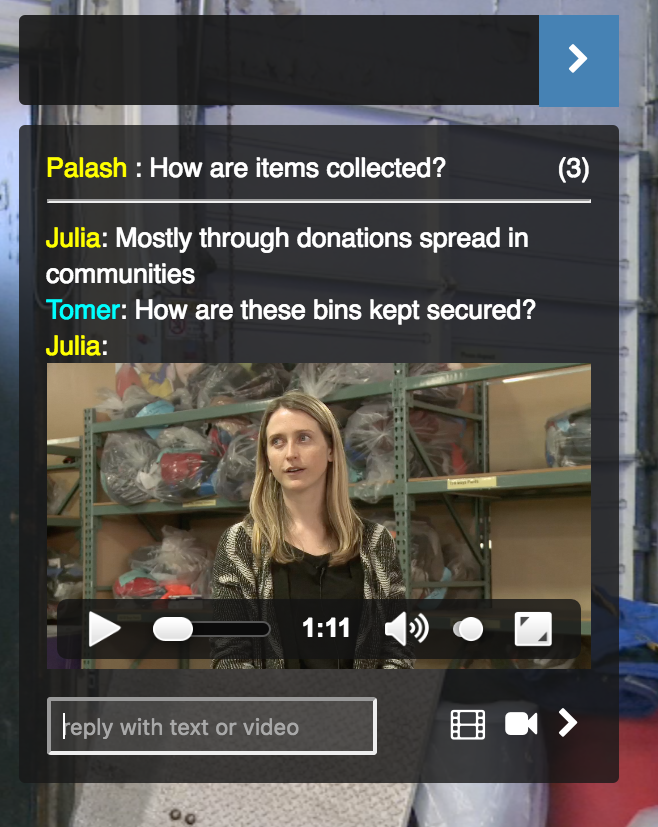
\includegraphics[width=2in]{figures/commentthread.png}
      \caption{This is How - Comment Thread}
      \label{fig_comment_thread}
   \end{figure}

Comments are collapsible into discussion threads. These threads provide a mechanism for other participants and the publisher of the story to explain, clarify and drill down into the story. These threads allow both textual and video replies for the sake of expressiveness. Videos replies can be either pre-recorded or recorded on the spot via a webcam. 

% Figure: Seekbar

All of the comments are displayed as semi-transparent blocks on the seek bar and on mouse hover will display the respective comment. At a glance, it is evident which areas of the video are active in terms of discussion and provides a seeking mechanism for the author and other participants.  

\subsection{Idea Pad}

   \begin{figure}[thpb]
      \centering
      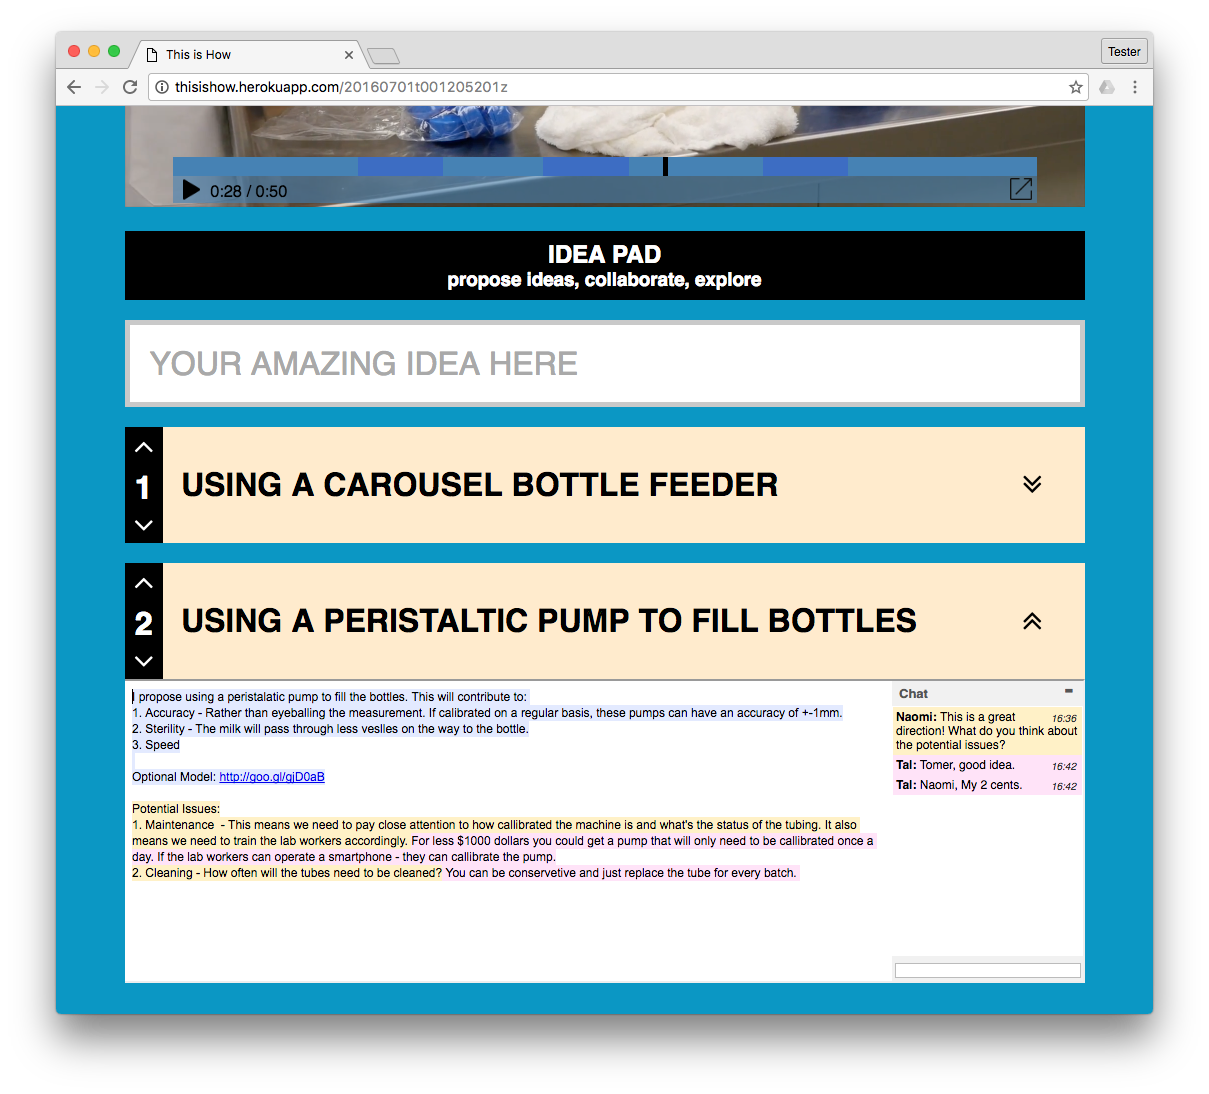
\includegraphics[width=\textwidth]{figures/ideapad-collapsed.png}
      \caption{This is How - Idea Pad}
      \label{fig_comment_thread}
   \end{figure}

The idea pad accommodates brainstorming by allowing participants to suggest ideas. Initially, an idea is entered as an idea title. Rather than discussing these ideas as simple conversations, they collapse into collaborative documents which any user can share and help evolve. These documents also contains a discussion pane in order not to pollute the document with traditional conversation. 

These ideas can be voted up and down by other participants, a common practice in Q\&A services\cite{stackoverflow}\cite{quora} that allows for the community to bubble up the worthy ideas.   